\documentclass[border=2]{standalone}
\usepackage[utf8]{inputenc}

\usepackage{flowchart}
\usetikzlibrary{arrows}

\newcommand{\red}[1]{{\color{red}$#1$}}

\begin{document}
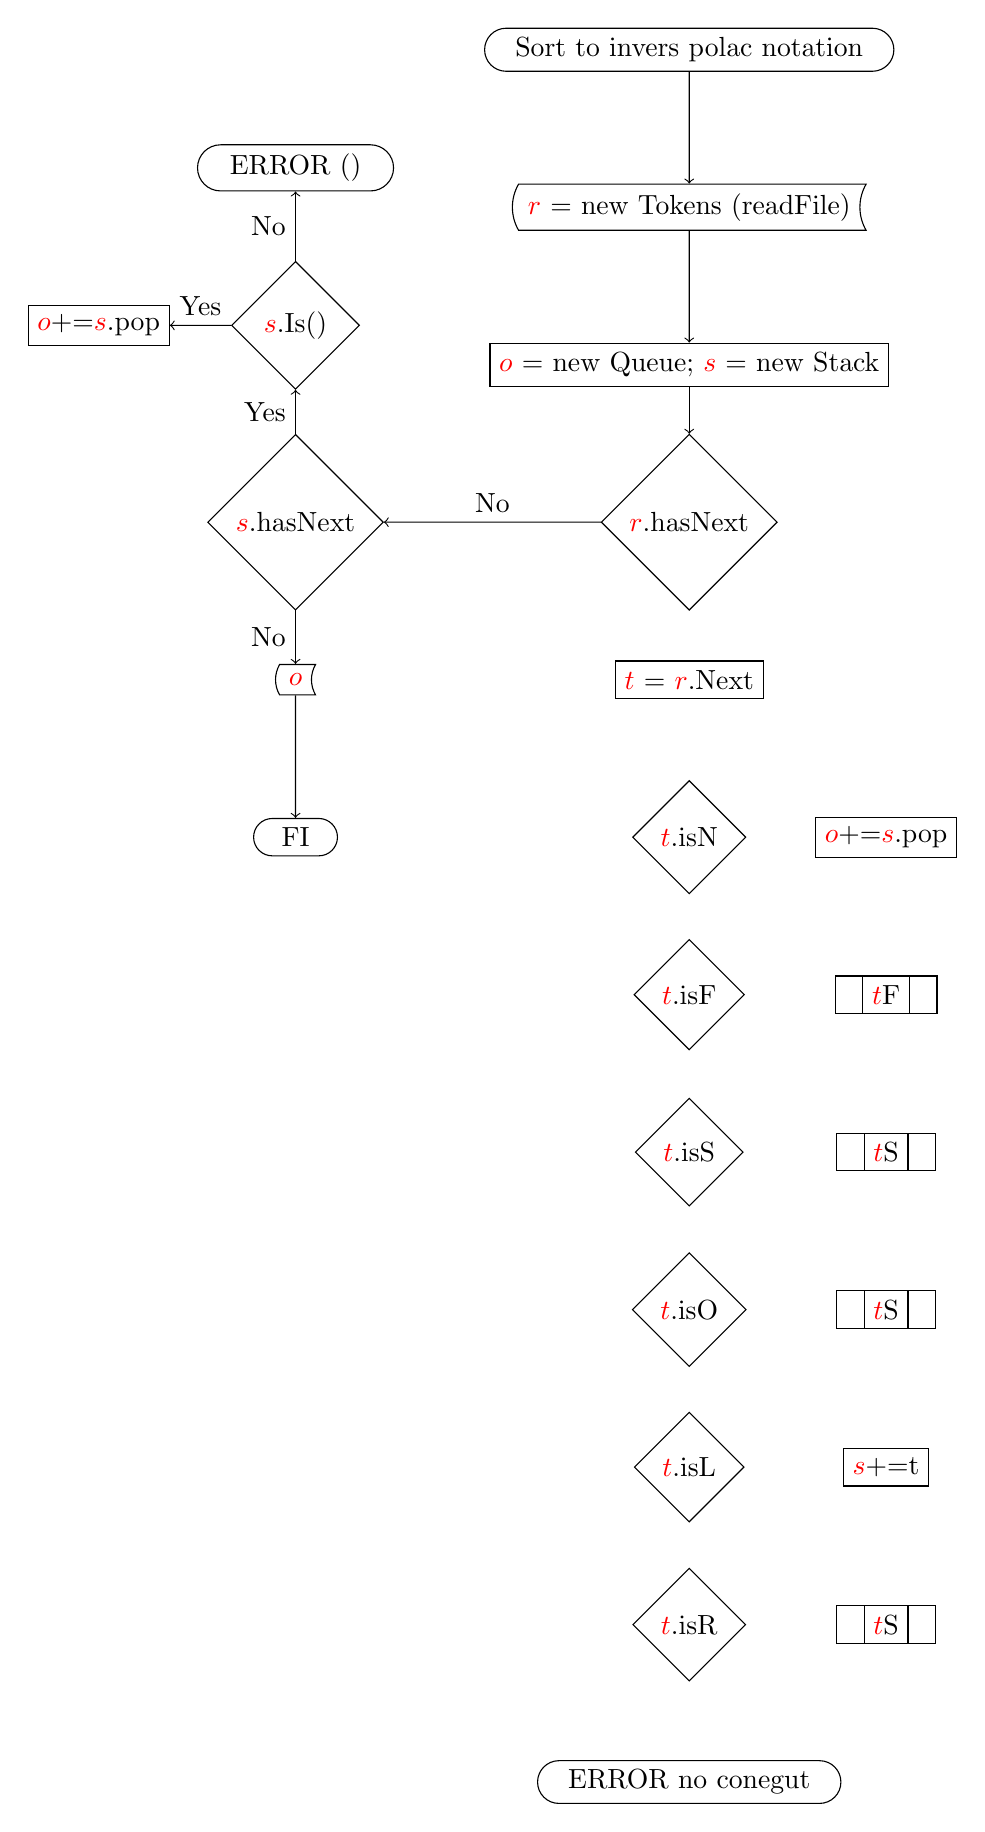
\begin{tikzpicture}[node distance = 2cm, auto]
% process/ decision/ terminal/ predproc/ storage/

%%%%%%%%%%%%%%%%%%%%%%%%%%%%%%%%%%%%%%%%%%%%%%%%%%%%%%%%%%%%%%%%%%%%%%%%%%%%%%%%%%%%%%%%%%%%%%%%%%%%%%%%%%%%%%%%%%%%%%%%%%%%%%%%
% Nucli, principal
%%%%%%%%%%%%%%%%%%%%%%%%%%%%%%%%%%%%%%%%%%%%%%%%%%%%%%%%%%%%%%%%%%%%%%%%%%%%%%%%%%%%%%%%%%%%%%%%%%%%%%%%%%%%%%%%%%%%%%%%%%%%%%%%
\node [draw, terminal] (IniciSatanicContraEvangelics) {Sort to invers polac notation};
\node [draw, storage, below of=IniciSatanicContraEvangelics] (readInfixDirtyNotation) {\red{r} = new Tokens (readFile)};
\node [draw, process, below of=readInfixDirtyNotation] (declareQueueAndStack) {\red{o} = new Queue; \red{s} = new Stack};
\node [draw, decision, below of=declareQueueAndStack] (mainWhile) {\red{r}.hasNext};
	\node [draw, decision, left of=mainWhile, node distance=5cm] (StackEmptyToEnd) {\red{s}.hasNext};
	\node [draw, decision, above of=StackEmptyToEnd, node distance=2.5cm] (StackEndnoLikeParentesis) {\red{s}.Is()};
	\node [draw, terminal, above of=StackEndnoLikeParentesis] (ERROREndParentesis) {ERROR ()};
\node [draw, process, left of=StackEndnoLikeParentesis, node distance=2.5cm] (AfegintQuanAsseguratLikeEndParentesis) {\red{o}+=\red{s}.pop};
	\node [draw, storage, below of=StackEmptyToEnd] (GuardantResultat) {\red{o}};
	\node [draw, terminal, below of=GuardantResultat] (FinalEndingPrograma) {FI};
\node [draw, process, below of=mainWhile] (EaserForNotAlotTimePeek) {\red{t} = \red{r}.Next};
\node [draw, decision, below of=EaserForNotAlotTimePeek] (butIsNumber) {\red{t}.isN};
	\node [draw, process, right of=butIsNumber, node distance=2.5cm] (butIsNextNumber) {\red{o}+=\red{s}.pop};
\node [draw, decision, below of=butIsNumber] (butIsFuntion) {\red{t}.isF};
	\node [draw, predproc, right of=butIsFuntion, node distance=2.5cm] (butIsNextFuntion) {\red{t}F};
\node [draw, decision, below of=butIsFuntion] (butIsSeparator) {\red{t}.isS};
	\node [draw, predproc, right of=butIsSeparator, node distance=2.5cm] (butIsNextSeparator) {\red{t}S};
\node [draw, decision, below of=butIsSeparator] (butIsOperator) {\red{t}.isO};
	\node [draw, predproc, right of=butIsOperator, node distance=2.5cm] (butIsNextOperator) {\red{t}S};
\node [draw, decision, below of=butIsOperator] (butIsLeft) {\red{t}.isL};% left parentesis
	\node [draw, process, right of=butIsLeft, node distance=2.5cm] (butIsNextLeft) {\red{s}+=t};
\node [draw, decision, below of=butIsLeft] (butIsRight) {\red{t}.isR};% right parentesis
	\node [draw, predproc, right of=butIsRight, node distance=2.5cm] (butIsNextRight) {\red{t}S};
\node [draw, terminal, below of=butIsRight] (butIsUnknow) {ERROR no conegut};
\draw[->] (IniciSatanicContraEvangelics)	-- (readInfixDirtyNotation);
\draw[->] (readInfixDirtyNotation)	-- (declareQueueAndStack);
\draw[->] (declareQueueAndStack)	-- (mainWhile);
	\draw[->] (mainWhile)	-- node[anchor=south] {No} (StackEmptyToEnd);
	\draw[->] (StackEmptyToEnd)	-- node[anchor=east] {Yes} (StackEndnoLikeParentesis);
	\draw[->] (StackEndnoLikeParentesis)	-- node[anchor=east] {No} (ERROREndParentesis);
	\draw[->] (StackEndnoLikeParentesis)	-- node[anchor=south] {Yes} (AfegintQuanAsseguratLikeEndParentesis);
	\draw[->] (StackEmptyToEnd)	-- node[anchor=east] {No} (GuardantResultat);
	\draw[->] (GuardantResultat)	-- (FinalEndingPrograma);

\end{tikzpicture}
\end{document}

Llegenda:
()	Parentesis
o	output
t	token
r	tokens
s	stack
L	Left parentesis
R	Right parentesis
N	Number
F	Funtion
S	Separator
O	Operation

Per entendre la magia, una funcio acaba sempre amb (, Ex: v(, ve a ser un vector. % fora pensava amb -, v- etc
llavors entent v( com a parentesis obert
	Aquest tindra un valor, igual que +, -, *, ... El qual indicara si es definit o indefinit, el nombre d'elements d'aquest

Exemple
Indefinit (,)
v( 4 , 6 , 7 ) => , 4 6 7 v-
Definit
M2i2( 1 , 4 , 8 , 9 ) => 1 4 8 9 M2i2-
